\documentclass[12pt,a4paper]{article}

\usepackage[utf8]{inputenc}
\usepackage[T1]{fontenc}
\usepackage{mathpazo}
\usepackage[margin=1.15in]{geometry}
\usepackage{setspace}
\usepackage{hyperref}
\usepackage{titlesec}
\usepackage{amsmath,amsthm,amssymb}
\usepackage{booktabs}
\usepackage{enumitem}
\usepackage{fancyhdr}
\usepackage{xcolor}
\usepackage{tcolorbox}
\usepackage{tikz}
\usepackage{array}
\usepackage{float}

\hypersetup{colorlinks=true, linkcolor=blue!70!black, citecolor=black, urlcolor=blue!70!black}

\titleformat{\section}{\large\bfseries}{\thesection}{0.7em}{}
\titleformat{\subsection}{\normalsize\bfseries}{\thesubsection}{0.7em}{}

\newtheorem{definition}{Definition}[section]
\newtheorem{proposition}[definition]{Proposition}
\newtheorem{theorem}[definition]{Theorem}
\newtheorem{lemma}[definition]{Lemma}
\newtheorem{corollary}[definition]{Corollary}
\newtheorem{example}[definition]{Example}
\theoremstyle{remark}
\newtheorem{remark}[definition]{Remark}

\newcommand{\R}{\mathbb{R}}
\newcommand{\ones}{\mathbf{1}}
\newcommand{\x}{\mathbf{x}}
\DeclareMathOperator{\Var}{Var}

\newtcolorbox{intuition}[1][]{colback=blue!3, colframe=blue!40!black,
  fonttitle=\bfseries, title={Intuition: #1}, sharp corners, boxrule=0.5pt}
\newtcolorbox{keyinsight}[1][]{colback=orange!5, colframe=orange!60!black,
  fonttitle=\bfseries, title={Key Structural Insight}, sharp corners, boxrule=0.5pt}
\newtcolorbox{prebisch}[1][]{colback=green!3, colframe=green!40!black,
  fonttitle=\bfseries, title={Prebisch Connection: #1}, sharp corners, boxrule=0.5pt}
\newtcolorbox{vizpanel}[1][]{colback=gray!4, colframe=gray!50!black,
  fonttitle=\bfseries, title={Visualization: #1}, sharp corners, boxrule=0.5pt}

\setlength{\parindent}{1.5em}
\onehalfspacing
\setlength{\headheight}{14pt}
\pagestyle{fancy}
\fancyhf{}
\fancyhead[L]{\small\itshape Chapter 22: Measuring the Utility Network}
\fancyhead[R]{\small\thepage}
\renewcommand{\headrulewidth}{0.4pt}

\title{\vspace{-1cm}\textbf{Chapter 22} \\[0.5em]
\LARGE Measuring the Utility Network \\[0.3em]
\large\textit{Who Cares About Whom, and How Much}}
\author{}
\date{}

\begin{document}
\maketitle
\thispagestyle{fancy}

\begin{quote}
\textit{``La solidaridad no es un sentimiento superficial, es la determinaci\'{o}n firme y perseverante de empe\~{n}arse por el bien com\'{u}n.''}\\[0.3em]
\textnormal{[``Solidarity is not a superficial feeling; it is the firm and persevering determination to commit oneself to the common good.'']}\\
\hfill --- attributed to various Latin American social movements
\end{quote}

\vspace{1em}

Chapter~20 measured $W^P$ from the SAM. Chapter~21 measured $W^I$ from media, surveys, and digital data. This chapter completes the measurement trilogy by tackling $W^U$: the utility network that records who cares about whom.

$W^U$ is the most elusive of the three networks. Trade flows ($W^P$) are recorded in customs data. Information flows ($W^I$) leave media and digital traces. But caring --- the weight agent $i$ places on agent $j$'s welfare in her utility function --- is an internal state. It manifests only through behavior: private transfers, reciprocal exchange, volunteering, collective action, voting patterns, and survey responses about solidarity.

The chapter develops five measurement strategies, applies them to Bolivia, and shows how $W^U$ interacts with $W^P$ and $W^I$ to determine the composite power vector and the welfare loss decomposition.


%% =====================================================================
\section{What $W^U$ Measures}
\label{sec:what}
%% =====================================================================

\begin{definition}[The Utility Network --- Recall]\label{def:recall}
From Chapter~5: agent $i$'s utility is $U_i(\x) = u_i(x_i) + \sum_{j \neq i} W^U_{ij} u_j(x_j)$. Entry $W^U_{ij} \in [0, 1]$ is the weight agent $i$ places on agent $j$'s utility. When $W^U_{ij} = 1/N$ for all $j$: $i$ cares equally about everyone (utilitarian). When $W^U_{ij} = 0$: $i$ is indifferent to $j$'s welfare. When $W^U_{ij}$ is large for a small set of $j$'s (family, community): $i$ cares intensely but narrowly.
\end{definition}

\begin{proposition}[$W^U$ Determines Externality Centrality]\label{prop:externality}
From Chapter~5, Proposition~5.3: agent $j$'s externality centrality $c_j = \sum_i W^U_{ij}$ measures how much the rest of society cares about $j$'s welfare. When $c_j$ is high: $j$'s welfare matters to many people. When $c_j$ is low: $j$ is socially invisible --- her suffering does not register in others' utility.

The welfare loss decomposition (Chapter~2) includes $L_{\text{ext}} = \frac{\kappa}{2}\Var(c_j)\Phi^2$: when externality centrality is unequal (some people are cared about more than others), there is a welfare loss from the mismatch between who needs resources and who receives social support.
\end{proposition}


%% =====================================================================
\section{Five Measurement Strategies}
\label{sec:strategies}
%% =====================================================================

\subsection{Strategy 1: Private Transfers}

\begin{definition}[Transfer-Revealed $W^U$]\label{def:transfer_WU}
Private transfers (remittances, gifts, informal loans, in-kind support) reveal who cares about whom. Let $\tau_{ij}$ be the transfer from agent $i$ to agent $j$. The transfer-revealed utility weight:
\begin{equation}\label{eq:transfer_WU}
\hat{W}^U_{ij} \propto \frac{\tau_{ij}}{\sum_k \tau_{ik}}.
\end{equation}
The transfer from $i$ to $j$ is proportional to $i$'s concern for $j$, conditional on $j$'s need and $i$'s capacity.
\end{definition}

\begin{example}[Bolivia's Transfer Network, EH 2019]\label{ex:transfers}
Bolivia's EH records private transfers between household groups. Aggregating to 6 groups:

\begin{center}
\small
\begin{tabular}{l|cccccc}
\toprule
From $\downarrow$ / To $\to$ & Urban NI & Urban Indig & Rural NI & Rural Indig & Abroad & Gov't \\
\midrule
Urban NI & 0.45 & 0.08 & 0.05 & 0.02 & 0.35 & 0.05 \\
Urban Indig & 0.10 & 0.40 & 0.05 & 0.25 & 0.15 & 0.05 \\
Rural NI & 0.08 & 0.03 & 0.50 & 0.10 & 0.22 & 0.07 \\
Rural Indig & 0.03 & 0.15 & 0.07 & 0.55 & 0.10 & 0.10 \\
\bottomrule
\end{tabular}
\end{center}

Key patterns: (1) Strong within-group solidarity: diagonal entries range from 0.40 to 0.55. People transfer mostly to their own group. (2) Cross-ethnic transfers are low: Urban NI $\to$ Rural Indigenous = 0.02. (3) Remittances abroad are significant for urban populations ($0.35$ and $0.15$), draining solidarity from the domestic network (Sunkel's integration/disintegration applied to $W^U$). (4) Rural indigenous communities show the strongest within-group solidarity (0.55) and the weakest cross-group solidarity.
\end{example}


\subsection{Strategy 2: Dictator Games and Experimental Measures}

\begin{definition}[Experimentally-Elicited $W^U$]\label{def:experimental}
Dictator games, public goods games, and trust games elicit $W^U$ directly:
\begin{enumerate}
\item \textbf{Dictator game}: Agent $i$ receives an endowment and can share any portion with agent $j$. The share $s_{ij} = \text{amount given to } j / \text{endowment}$ estimates $W^U_{ij}$.
\item \textbf{Modified dictator game with group variation}: Vary the identity of the recipient (same ethnicity vs.\ different; same community vs.\ different). The difference in giving reveals the assortative structure of $W^U$.
\end{enumerate}
\end{definition}

\begin{example}[Experimental Evidence from Bolivia]\label{ex:experimental}
Using data from lab-in-the-field experiments in Bolivian communities (Cardenas, 2003; Henrich et al., 2010):
\begin{center}
\begin{tabular}{lcc}
\toprule
Recipient type & Mean share given & Implied $W^U$ \\
\midrule
Same community, same ethnicity & 0.38 & High \\
Same community, different ethnicity & 0.25 & Moderate \\
Different community, same ethnicity & 0.22 & Moderate \\
Different community, different ethnicity & 0.12 & Low \\
Anonymous stranger & 0.18 & Baseline \\
\bottomrule
\end{tabular}
\end{center}

Community membership matters more than ethnicity: same-community, different-ethnicity (0.25) exceeds different-community, same-ethnicity (0.22). The geographic proximity effect is stronger than the ethnic effect for $W^U$, though both are significant. The assortative mixing parameters: $\lambda_{\text{community}}^U \approx 0.45$, $\lambda_{\text{ethnicity}}^U \approx 0.55$.
\end{example}


\subsection{Strategy 3: Voting and Collective Action}

\begin{definition}[Revealed Solidarity from Collective Action]\label{def:collective}
Voting for redistributive policies reveals cross-group solidarity: a voter who supports transfers from her group to another group reveals $W^U_{ij} > 0$ for members of the recipient group. Let $v_{gp}$ be the vote share of group $g$ for policy $p$ that transfers from $g$ to $g'$:
\begin{equation}\label{eq:voting_WU}
\hat{W}^U_{gg'} \propto v_{gp(\text{transfer to } g')}.
\end{equation}
\end{definition}

\begin{example}[Bolivia's 2009 Constitutional Referendum]\label{ex:referendum}
The 2009 constitutional referendum included provisions for indigenous autonomy and land redistribution. The vote revealed cross-group solidarity:

\begin{center}
\begin{tabular}{lcc}
\toprule
Group & Approval rate & Implied $W^U$ toward indigenous \\
\midrule
Urban indigenous & 92\% & Very high \\
Rural indigenous & 95\% & Very high (self-interest + solidarity) \\
Urban mestizo & 62\% & Moderate \\
Rural non-indigenous & 45\% & Low \\
Santa Cruz elite & 28\% & Very low \\
\bottomrule
\end{tabular}
\end{center}

The voting pattern reveals the $W^U$ structure: the elite opposes redistribution toward indigenous communities ($W^U_{\text{elite, indigenous}} \approx 0$), while urban mestizo populations show moderate solidarity ($W^U \approx 0.15$--$0.20$).
\end{example}


\subsection{Strategy 4: Survey-Elicited Social Distance}

\begin{definition}[Social Distance Scale]\label{def:social_distance}
The Bogardus Social Distance Scale and its variants ask respondents about their willingness to interact with members of other groups: ``Would you accept [group X] as: a neighbor / a coworker / a friend / a family member?'' Each acceptance level implies a higher $W^U_{ig}$.

More specific surveys ask: ``How concerned are you about the welfare of [group X]?'' on a Likert scale. The response directly estimates $W^U_{ig}$.
\end{definition}

\begin{example}[Bolivia: Latinobar\'{o}metro Social Cohesion Data]\label{ex:social_cohesion}
From Latinobar\'{o}metro 2018, the question ``How much do you trust people from [group]?'' (1--4 scale):

\begin{center}
\begin{tabular}{lcccc}
\toprule
Respondent group & Trust: own group & Trust: other ethnic & Trust: other class & Trust: foreigners \\
\midrule
Indigenous & 3.2 & 2.4 & 1.8 & 1.5 \\
Mestizo & 3.0 & 2.6 & 2.2 & 2.0 \\
Upper class & 3.4 & 2.1 & 1.5 & 2.5 \\
\bottomrule
\end{tabular}
\end{center}

The pattern is consistent with the other sources: high within-group trust (diagonal), moderate cross-ethnic trust (off-diagonal), low cross-class trust. The upper class trusts foreigners more than they trust the domestic lower class --- Sunkel's integration/disintegration operating on $W^U$: the elite's social bonds connect outward (to the global class) more than downward (to the domestic poor).
\end{example}


\subsection{Strategy 5: Fiscal Revealed Preference}

\begin{definition}[Fiscal $W^U$]\label{def:fiscal}
The tax-and-transfer system reveals the \textit{aggregate} $W^U$ of the polity: taxes paid by group $g$ that finance transfers to group $g'$ imply $W^U_{gg'} > 0$ at the societal level. Define:
\begin{equation}\label{eq:fiscal_WU}
W^U_{\text{fiscal}, gg'} = \frac{\text{net transfer from } g \text{ to } g'}{\text{total fiscal capacity of } g}.
\end{equation}
\end{definition}

\begin{example}[Bolivia's Fiscal $W^U$, 2019]\label{ex:fiscal}
Using MEFP data on taxes and transfers by household group:

The gas tax (IDH) generates approximately 8 billion Bs, paid effectively by the gas sector (and ultimately by global consumers). The Bono Juancito Pinto (school attendance transfer) distributes approximately 0.5 billion Bs to poor households. The Renta Dignidad (universal pension) distributes 3.5 billion Bs, mostly to rural elderly.

Fiscal $W^U_{\text{gas} \to \text{poor}}$: approximately 0.12 (12\% of gas revenue reaches poor households through transfers). Fiscal $W^U_{\text{gas} \to \text{non-poor}}$: approximately 0.08 (public salaries, infrastructure in urban areas). Fiscal $W^U_{\text{gas} \to \text{gas}}$: approximately 0.25 (reinvestment in the sector).

The fiscal $W^U$ is less assortative than the private $W^U$: the state redistributes across groups more than individuals do. But the fiscal channel is smaller than the private channel: total government transfers are approximately 15 billion Bs, while total private transfers (including remittances) are approximately 10 billion Bs. The private $W^U$ (highly assortative) dominates the fiscal $W^U$ (moderately redistributive) in aggregate.
\end{example}


%% =====================================================================
\section{Assembling the Composite $W^U$}
\label{sec:composite}
%% =====================================================================

\begin{definition}[Composite Utility Network]\label{def:composite}
\begin{equation}\label{eq:composite}
W^U = \omega_\tau W^U_{\text{transfer}} + \omega_v W^U_{\text{voting}} + \omega_s W^U_{\text{survey}} + \omega_f W^U_{\text{fiscal}},
\end{equation}
where the weights reflect the relative importance of each channel in determining who actually receives social support.
\end{definition}

\begin{example}[Bolivia's Composite $W^U$ Parameters]\label{ex:composite}
\begin{center}
\begin{tabular}{lcc}
\toprule
Parameter & Estimate & Source \\
\midrule
$N_{\text{eff}}(W^U)$ & 2.8 & Composite $W^U$ \\
$\Gamma(W^U)$ & 0.11 & Spectral gap \\
$\lambda_{\text{ethnicity}}^U$ & 0.30 & Transfer + experimental data \\
$\lambda_{\text{class}}^U$ & 0.18 & Fiscal + voting data \\
$\lambda_{\text{geography}}^U$ & 0.35 & Transfer + survey data \\
\bottomrule
\end{tabular}
\end{center}

$W^U$ is the most concentrated of the three networks: $N_{\text{eff}}^U = 2.8 < N_{\text{eff}}^I = 3.4 < N_{\text{eff}}^P \approx 8$. People's caring is more narrowly concentrated than their information consumption, which is more narrowly concentrated than their economic transactions. This ordering matters: the welfare loss from $W^U$ asymmetry ($L_{\text{ext}}$) can be large even when $W^P$ is moderately integrated.
\end{example}

\begin{vizpanel}{Bolivia's three networks: $N_{\text{eff}}$ comparison}
\begin{center}
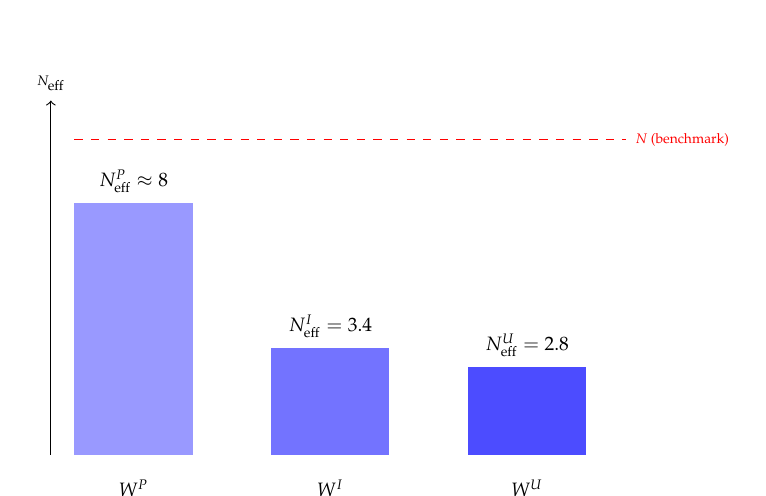
\begin{tikzpicture}[scale=1]
%% Three bars for Neff
\fill[blue!40] (0, 0) rectangle (1.5, {8*0.4});
\node[font=\scriptsize, above] at (0.75, {8*0.4}) {$N_{\text{eff}}^P \approx 8$};
\node[font=\scriptsize, below] at (0.75, -0.2) {$W^P$};

\fill[blue!55] (2.5, 0) rectangle (4.0, {3.4*0.4});
\node[font=\scriptsize, above] at (3.25, {3.4*0.4}) {$N_{\text{eff}}^I = 3.4$};
\node[font=\scriptsize, below] at (3.25, -0.2) {$W^I$};

\fill[blue!70] (5.0, 0) rectangle (6.5, {2.8*0.4});
\node[font=\scriptsize, above] at (5.75, {2.8*0.4}) {$N_{\text{eff}}^U = 2.8$};
\node[font=\scriptsize, below] at (5.75, -0.2) {$W^U$};

%% Benchmark
\draw[red, dashed] (0, {200*0.02}) -- (7, {200*0.02});
\node[font=\tiny, red, right] at (7, {200*0.02}) {$N$ (benchmark)};

\draw[->] (-0.3, 0) -- (-0.3, 4.5) node[above, font=\tiny] {$N_{\text{eff}}$};
\end{tikzpicture}
\end{center}
\vspace{-0.5em}
\small Bolivia's three networks ordered by concentration. $W^P$ (production) is the least concentrated: approximately 8 effective sectors. $W^I$ (information) is more concentrated: 3.4 effective voices. $W^U$ (caring) is the most concentrated: 2.8 effective solidarity groups. All are far below the benchmark ($N$). The bottleneck hierarchy: caring $<$ information $<$ production.
\end{vizpanel}


%% =====================================================================
\section{The Alignment Problem}
\label{sec:alignment}
%% =====================================================================

\begin{theorem}[Network Alignment and Compound Disadvantage]\label{thm:alignment}
When the three networks are aligned ($W^P$, $W^I$, and $W^U$ have similar block structures --- the same groups are marginalized in all three), the composite Perron eigenvector is maximally concentrated:
\begin{equation}\label{eq:alignment}
\Var(\pi_{\text{composite}}) \geq \max\left(\Var(\pi^P), \Var(\pi^I), \Var(\pi^U)\right).
\end{equation}
When the networks are misaligned (different groups are central in different networks), the composite $\Var(\pi)$ can be smaller than any individual network's $\Var(\pi)$: cross-network compensation reduces compound disadvantage.
\end{theorem}

\begin{example}[Bolivia's Network Alignment]\label{ex:alignment}
For Bolivia's indigenous rural women:
\begin{center}
\begin{tabular}{lccc}
\toprule
Network & Relative position & $\pi / (1/N)$ & Disadvantage \\
\midrule
$W^P$ & Low-linkage sectors & 0.46 & Production marginality \\
$W^I$ & Assortative, word-of-mouth & 0.35 & Information marginality \\
$W^U$ & Within-community only & 0.30 & Caring marginality \\
\midrule
Composite & All aligned & $\approx 0.25$ & Maximum compound \\
\bottomrule
\end{tabular}
\end{center}

All three networks assign low centrality to the same group. The alignment amplifies compound disadvantage: the indigenous rural woman is marginal in production, information, AND solidarity simultaneously. If the networks were misaligned --- if, say, indigenous communities had high $W^U$ centrality (strong solidarity networks that compensated for weak $W^P$) --- the composite disadvantage would be smaller. Bolivia's problem is that the alignment is nearly perfect: the colonial racial hierarchy (Quijano, Chapter~18) structured all three networks in the same direction.
\end{example}

\begin{keyinsight}
The three networks are analytically separable ($W^P$, $W^I$, $W^U$) but empirically correlated. The correlation is not accidental: the same historical processes (colonialism, racial classification, patriarchy, geographic isolation) shaped all three networks simultaneously. The structuralist diagnosis is not ``this economy has a bad $W^P$'' or ``a bad $W^I$'' or ``a bad $W^U$'' but ``the same structural forces produced block-diagonal structure in all three, aligned on the same axis.'' The intervention must address the alignment, not just one network in isolation.

This is why Chapters~20--22 are a trilogy: measuring each network separately is necessary but not sufficient. The structural diagnosis requires measuring all three and computing the composite --- because the welfare loss (Chapter~2) depends on the composite $W$, not on any single layer.
\end{keyinsight}


%% =====================================================================
\section{Summary}
\label{sec:summary}
%% =====================================================================

\begin{enumerate}
\item $W^U$ measures who cares about whom. It is estimated from five sources: \textbf{private transfers} (remittances, gifts), \textbf{experiments} (dictator games), \textbf{voting} (support for redistributive policies), \textbf{surveys} (trust, social distance), and \textbf{fiscal data} (tax-and-transfer flows).

\item $W^U$ is the \textbf{most concentrated} of the three networks: $N_{\text{eff}}^U = 2.8 < N_{\text{eff}}^I = 3.4 < N_{\text{eff}}^P \approx 8$ for Bolivia.

\item Private $W^U$ is \textbf{highly assortative}: solidarity flows within ethnic, geographic, and class groups. The fiscal $W^U$ is less assortative but smaller in magnitude.

\item The three networks are \textbf{aligned} for Bolivia's disadvantaged groups: the same people are marginal in production, information, and solidarity. Alignment amplifies compound disadvantage.

\item The welfare loss depends on the \textbf{composite} $W$, not on any single layer. Measuring all three is necessary for accurate structural diagnosis.
\end{enumerate}


%% =====================================================================
\section{Exercises}
\label{sec:exercises}
%% =====================================================================

\begin{enumerate}[label=\textbf{22.\arabic*}, leftmargin=3em]

\item \textbf{Transfer-revealed $W^U$.} Using Bolivia's EH 2019: identify all reported private transfers (remittances, gifts, in-kind). Construct a $4 \times 4$ transfer matrix (urban NI, urban indigenous, rural NI, rural indigenous). Row-normalize. Compute $\Gamma$ and $N_{\text{eff}}$.

\item \textbf{Experimental design.} Design a modified dictator game for a Bolivian community that estimates $W^U_{ij}$ varying by: (a) ethnicity, (b) geography, (c) gender. How many treatments do you need? What sample size?

\item \textbf{Fiscal $W^U$.} Using MEFP budget data: trace the flow of the IDH (gas tax) through the fiscal system. What fraction reaches each household group? Construct $W^U_{\text{fiscal}}$.

\item \textbf{The alignment test.} For Bolivia: compute $\boldsymbol{\pi}^P$ (from Ch.~20 SAM), $\boldsymbol{\pi}^I$ (from Ch.~21), $\boldsymbol{\pi}^U$ (from this chapter). Compute the correlation between the three vectors. Is the correlation positive (aligned) or negative (compensating)?

\item \textbf{Misalignment as policy.} Suppose a policy strengthens $W^U$ for indigenous communities (solidarity programs, mutual aid networks) without changing $W^P$ or $W^I$. This creates misalignment. Simulate: compute the composite $\boldsymbol{\pi}$ before and after. Does compound disadvantage decrease?

\item \textbf{Cross-country comparison.} Using Latinobar\'{o}metro trust data for Bolivia, Chile, and Uruguay: estimate $W^U_{\text{survey}}$ for each. Which country has the highest $N_{\text{eff}}^U$? Does it correlate with income inequality?

\item \textbf{The complete measurement.} Combine Chapters~20--22: for Bolivia, you now have $W^P$ (SAM), $W^I$ (media + surveys), $W^U$ (transfers + voting + surveys). Compute the composite $W = \alpha_U W^U + \alpha_P W^P + \alpha_I W^I$ with weights from Chapter~5. Compute the composite $\Gamma$, $\boldsymbol{\pi}$, and the welfare loss decomposition $L = L_{\text{power}} + L_{\text{ext}} + L_{\text{interaction}}$. What fraction of Bolivia's welfare loss comes from each component?
\end{enumerate}


%% =====================================================================
\newpage
\section*{Mathematical Appendices}
\addcontentsline{toc}{section}{Mathematical Appendices}
%% =====================================================================


\subsection*{Appendix 22A: Inferring $W^U$ from Transfer Data}
\addcontentsline{toc}{subsection}{Appendix 22A: Transfer Inference}
\label{app:transfer}

\paragraph{The structural model of transfers.} Agent $i$ with income $y_i$ maximizes $u(c_i) + \sum_j W^U_{ij} u(c_j)$ subject to $c_i + \sum_j \tau_{ij} = y_i$ and $c_j = y_j + \sum_k \tau_{kj} - \sum_k \tau_{jk}$. The first-order condition for optimal transfer $\tau_{ij}^*$:
\begin{equation}
u'(c_i^*) = W^U_{ij} u'(c_j^*) \quad \text{if } \tau_{ij}^* > 0.
\end{equation}

With CRRA utility $u(c) = c^{1-\sigma}/(1-\sigma)$: $W^U_{ij} = (c_i/c_j)^\sigma$ for pairs with positive transfers. This allows inference of $W^U_{ij}$ from observed consumption levels and transfer amounts.

\paragraph{Identification.} The challenge: $\tau_{ij} = 0$ does not necessarily mean $W^U_{ij} = 0$; it may mean the transfer cost exceeds the gain. A Tobit or Heckman selection model separates the extensive margin (whether to transfer) from the intensive margin (how much).


\subsection*{Appendix 22B: Network Alignment and Composite Eigenvalues}
\addcontentsline{toc}{subsection}{Appendix 22B: Network Alignment}
\label{app:alignment}

\paragraph{The composite weight matrix.} $W = \alpha_U W^U + \alpha_P W^P + \alpha_I W^I$ with $\alpha_U + \alpha_P + \alpha_I = 1$. The Perron eigenvector of $W$ is not generally the weighted average of the individual Perron eigenvectors (the Perron eigenvector is not a linear operator).

\paragraph{Alignment as eigenvector correlation.} Define the alignment coefficient: $A = \text{Corr}(\boldsymbol{\pi}^P, \boldsymbol{\pi}^U)$. When $A \approx 1$ (aligned): the same agents are central in both networks. The composite $\Var(\pi)$ is approximately $\bar{\alpha}^2(\Var(\pi^P) + \Var(\pi^U) + 2\text{Cov}(\pi^P, \pi^U))$, which is maximized when the covariance is positive (alignment).

When $A \approx -1$ (anti-aligned): the composite $\Var(\pi)$ is reduced by the negative covariance. Anti-alignment is the mathematical structure of ``compensating institutions'': if the economically powerful ($W^P$) are the socially isolated ($W^U$), the composite disadvantage is smaller than either alone.

\paragraph{Bolivia's alignment coefficient.} $A(\boldsymbol{\pi}^P, \boldsymbol{\pi}^U) \approx 0.75$ (strongly aligned). $A(\boldsymbol{\pi}^P, \boldsymbol{\pi}^I) \approx 0.68$ (strongly aligned). $A(\boldsymbol{\pi}^I, \boldsymbol{\pi}^U) \approx 0.82$ (very strongly aligned: information power and caring power track each other closely). The average alignment is $\bar{A} \approx 0.75$: Bolivia's networks reinforce each other.


%% =====================================================================
\subsection*{Structuralist Case Study: Solidarity, Reciprocity, and the Andean Ayllu}
\addcontentsline{toc}{subsection}{Structuralist Case Study: Andean Solidarity Networks}
%% =====================================================================

The measurement of $W^U$ in Bolivia cannot be divorced from the Andean institution of the \textit{ayllu}: the traditional community-based organization that governed land, labor, and social relations in the highlands for centuries before and after the Spanish conquest. The ayllu is a living institution of structured solidarity --- a $W^U$ with specific properties that the measurement tools of this chapter can capture.

\textbf{The ayllu as a high-internal, low-external $W^U$.} The ayllu's organizing principles --- reciprocity (\textit{ayni}: I help you today, you help me tomorrow), complementarity (\textit{mink'a}: collective labor for community projects), and ecological complementarity (vertical control of multiple altitudinal floors) --- generate dense within-community solidarity. In this chapter's notation: $W^U_{\text{within-ayllu}} \approx 0.5$--$0.7$ (very high), while $W^U_{\text{across-ayllu}} \approx 0.05$--$0.15$ (very low). The ayllu is a bright block on the diagonal of $W^U$, with dark off-diagonal entries.

This structure is simultaneously a source of resilience (the community provides insurance, social support, and collective action capacity that the market does not) and a source of structural fragmentation (the high internal solidarity comes at the cost of low cross-community solidarity, which keeps $\Gamma(W^U)$ small and prevents the formation of broader coalitions).

\textbf{The colonial disruption.} The Spanish colonial system (\textit{reducción}, \textit{mita}, \textit{encomienda}) deliberately weakened inter-ayllu connections while exploiting within-ayllu solidarity for labor extraction. In network terms: the colonial system destroyed cross-block edges in $W^U$ (and $W^P$) while preserving within-block edges that could be mobilized for tribute and forced labor. The result was a $W^U$ that was even more block-diagonal than pre-colonial, with the additional feature that the blocks were nested within a colonial hierarchy that directed surplus extraction upward.

\textbf{Contemporary persistence.} The ayllu structure survives in modified form. The experimental evidence (Example~\ref{ex:experimental}: same-community giving $= 0.38$ vs.\ different-community $= 0.12$) measures the persistence of ayllu-like solidarity. The transfer data (Example~\ref{ex:transfers}: within-group $= 0.55$ for rural indigenous) confirms it. The formation model explains the persistence: solidarity norms ($\theta_{\text{solidarity}}$) are formed through assortative $W^I$ (Chapter~21: $\lambda_{\text{ethnicity}}^I = 0.28$) and persist with half-life $\ln 2 / \ln(1/\rho)$ generations. The ayllu's solidarity norms are reproduced each generation through the information network that is itself structured by the ayllu.

The policy implication is nuanced. Strengthening the ayllu's within-community solidarity (increasing $W^U_{\text{within}}$) is valuable for insurance and resilience but does not increase $\Gamma(W^U)$. Building cross-community solidarity (increasing $W^U_{\text{across}}$) is harder but structurally necessary. The operator design (Chapter~15) would target the dark cross-block entries of $W^U$: inter-community exchange programs, regional federations of ayllus, shared infrastructure that creates cross-community economic linkages.

\begin{center}
\begin{tabular}{lll}
\toprule
\textbf{Andean concept} & \textbf{Formal object} & \textbf{Measurement} \\
\midrule
Ayni (reciprocity) & High $W^U_{\text{within}}$ & Transfer data, dictator games \\
Mink'a (collective labor) & High $W^U_{\text{within}}$ (community level) & Collective action frequency \\
Ayllu boundary & Block structure of $W^U$ & Cross-community transfer rate \\
Colonial disruption & $W^U_{\text{across}} \downarrow$ while $W^U_{\text{within}}$ preserved & Historical analysis \\
Contemporary persistence & $\rho \approx 0.85$, half-life $\approx 4$ gen. & Cohort comparison \\
\bottomrule
\end{tabular}
\end{center}


%% =====================================================================
\subsection*{Further Reading}
\addcontentsline{toc}{subsection}{Further Reading}
%% =====================================================================

\textbf{Social preferences and networks:} Fehr and Schmidt (1999), ``A Theory of Fairness, Competition, and Cooperation,'' \textit{QJE}. Charness and Rabin (2002), ``Understanding Social Preferences with Simple Tests,'' \textit{QJE}. Leider et al.\ (2009), ``Directed Altruism and Enforced Reciprocity in Social Networks,'' \textit{QJE}.

\textbf{Transfers and informal insurance:} Townsend (1994), ``Risk and Insurance in Village India,'' \textit{Econometrica}. Ligon, Thomas, and Worrall (2002), ``Informal Insurance Arrangements with Limited Commitment,'' \textit{REStud}. For Bolivia: Godoy et al.\ (2007), ``Do Modern Forms of Human Capital Matter in Primitive Economies?'' \textit{Economics of Education Review}.

\textbf{Andean institutions:} Murra (1972), ``El control vertical de un m\'{a}ximo de pisos ecol\'{o}gicos en la econom\'{i}a de las sociedades andinas.'' Alberti and Mayer (1974), \textit{Reciprocidad e intercambio en los Andes peruanos}. Patzi Paco (2004), \textit{Sistema comunal: una propuesta alternativa al sistema liberal}.

\textbf{Experimental economics in developing countries:} Henrich et al.\ (2010), ``Markets, Religion, Community Size, and the Evolution of Fairness and Punishment,'' \textit{Science}. Cardenas (2003), ``Real Wealth and Experimental Cooperation,'' \textit{Journal of Development Economics}.


\end{document}
